% % % % % % % % % % % % % % % % % % % % % % % % % % % % % % % % % % % % % % % % % % % %
%                                                                                     %
% Short Sectioned Assignment LaTeX Template Version 1.0 (5/5/12)                      %
% This template has been downloaded from: http://www.LaTeXTemplates.com               %
%                                                                                     %
% Original author:  Frits Wenneker (http://www.howtotex.com)                          %
%                                                                                     %
% Modified by: Fco Javier Sueza Rodríguez (fcosueza@disroot.org)                      %
%                                                                                     %
% Changes:                                                                            %
%	    - Custom Chapters, Sections and Subsections (titlesec package)                %
%           - Document type scrbook (oneside)                                         %
%           - Use babel-lang-spanish package and marvosym                             %
%           - Use hyperref, enumitem, tcolorbox and glossaries packages               %
%           - Use Time New Roman (mathptmx), Helvetic and Courier fonts               %
%                                                                                     %
% License: CC BY-NC-SA 3.0 (http://creativecommons.org/licenses/by-nc-sa/3.0/)        %
%                                                                                     %
% % % % % % % % % % % % % % % % % % % % % % % % % % % % % % % % % % % % % % % % % % % %

%-----------------------------------------------%
%	              Packages                  %
%-----------------------------------------------%

\documentclass[paper=a4, fontsize=11pt, oneside]{scrbook}

% ---- Text Input/Output ----- %

\usepackage[T1]{fontenc}
\usepackage[utf8]{inputenc}
\usepackage{mathptmx}
\usepackage[scaled=.92]{helvet}
\usepackage{courier}
\usepackage[indent=12pt]{parskip}

\usepackage{geometry}
\geometry{verbose,tmargin=3cm,bmargin=3cm,lmargin=2.6cm,rmargin=2.6cm}

% ---- Language ----- %

\usepackage[spanish]{babel}
\usepackage{marvosym}

% ---- Another packages ---- %

\usepackage{amsmath,amsfonts,amsthm}
\usepackage{graphics,graphicx}
\usepackage{titlesec}
\usepackage{fancyhdr}
\usepackage{tcolorbox}
\usepackage{hyperref}
\usepackage{enumitem}
\usepackage[automake]{glossaries}

%--------------------------------------------------------------------%
%                      Customizing Document                          %
%--------------------------------------------------------------------%


% ----------- Custom Chapters, Sections and Subsections -------------- %

\titleformat{\chapter}[display]
			{\bfseries\Huge}
			{Tema \ \thechapter} {0.5ex}
			{\vspace{1ex}\centering}

\titleformat{\section}[hang]
			{\bfseries\Large}
			{\thesection}{0.5em}{}

\titleformat{\subsection}[hang]
			{\bfseries\large}
			{\thesubsection}{0.5em}{}

\titleformat{\subsubsection}[hang]
			{\bfseries\large}
			{\thesubsubsection}{0.5em}{}

\hypersetup{
    colorlinks=true,
    linkcolor=black,
    urlcolor=magenta
}

% ------------------- Custom heaaders and footers ------------------- %

\pagestyle{fancyplain}

\fancyhead[]{}
\fancyfoot[L]{}
\fancyfoot[C]{}
\fancyfoot[R]{\thepage}

\renewcommand{\headrulewidth}{0pt} % Remove header underlines
\renewcommand{\footrulewidth}{0pt} % Remove footer underlines

\setlength{\headheight}{13.6pt} % Customize the height of the header

% --------- Numbering equations, figures and tables ----------------- %

\numberwithin{equation}{section} % Number equations within sections
\numberwithin{figure}{section} % Number figures within sections
\numberwithin{table}{section} % Number tables within sections

% ------------------------ New Commands ----------------------------- %

\newcommand{\horrule}[1]{\rule{\linewidth}{#1}} % Create horizontal rule command


%----------------------------------------------------------------------------------------
%	TÍTULO Y DATOS DEL ALUMNO
%----------------------------------------------------------------------------------------

\title{
\vspace{10ex}
\normalfont \normalsize
\huge \textbf{Documentación y Control de Versiones}
}
\author{Francisco Javier Sueza Rodríguez}
\date{\normalsize\today}

%----------------------------------------------------------------------------------------
%                                     DOCUMENTO
%----------------------------------------------------------------------------------------
\begin{document}


\maketitle

\thispagestyle{empty}

\vspace{65ex}

\begin{center}
    \begin{tabular}{l l}
        \textbf{Centro}: & IES Aguadulce \\
        \textbf{Ciclo Formativo}: & Desarrollo Aplicaciones Web (Distancia)\\
        \textbf{Asignatura}: & Despliegue de Aplicaciones Web\\
        \textbf{Tema}: & Tema 5 - Documentación y Control de Versiones\\
    \end{tabular}
\end{center}

\newpage

\tableofcontents

\newpage

\listoffigures

\newpage

\section{Actividad 1: phpDocumentor}
Este ejercicio relacionado con generación de documentación consistirá en los siguientes apartados :

\subsection{Actividad 1.1}
Instala la herramienta phpdocumentor en tu servidor Linux y comenta los aspectos más importantes de tal herramienta, así como las etiquetas principales que se usan.

\subsubsection{Solución}
En este ejercicio vamos a realizar la instalación de \textbf{phpDocumentor} en la distribución \textbf{Kubuntu 22.04} de Linux. Hay varios métodos para realizar la instalación, se puede hacer mediante \textbf{Docker}, usando \textbf{Phive} o \textbf{manualmente}. La instalación mediante composer no es recomendada por los desarrolladores de phpDocumentor, ya que hay una alta probabilidad de que se generen conflictos con otras librerías.

Nosotros hemos optado por la \textbf{opción de instalación manual}. Para ello, solo hemos tenido que descargar el \textbf{paquete de phpDocumentor} del repositorio de \href{https://github.com/phpDocumentor/phpDocumentor/releases}{repositorio de Github} de la aplicación, desde donde hemos descargado la \textbf{versión 3.4.3}.

Una vez descargada la versión simplemente le hemos \textbf{agregado permisos de ejecución} y la hemos movido al directorio \textit{/usr/local/bin}, para que se puede ejecutar desde cualquier parte del sistema, como podemos ver en la siguiente captura.

\begin{figure}[H]
\centering
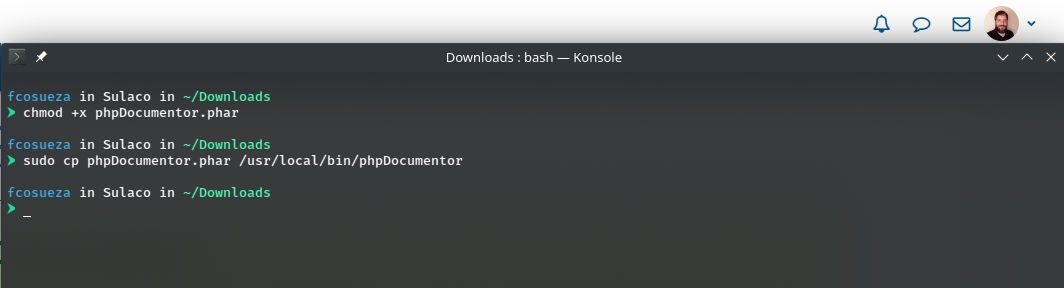
\includegraphics[scale=0.50]{installDoc.png}
\caption{Instalación de phpDocumentor}
\end{figure}

Actualmente, \textbf{phpDocumentor} es la aplicación más empleada para le \textbf{generación de documentación} en aplicaciones desarrolladas con PHP. Es el equivalente para PHP de \textbf{JavaDoc} para Java. Su instalación, como hemos visto, se hace de forma muy sencilla y su uso es igualmente sencillo, pudiendo ejecutarse desde la \textbf{línea de comandos}, la \textbf{interfaz web} o desde el \textbf{propio código PHP}.

Esta aplicación esta desarrollada en PHP y usa el lenguaje para la generación de la documentación, empleando para ello los \textbf{DocBlocks}, que son trozos de código incluidos en el código PHP que sirven para describir la funcionalidad, parámetros, valores devueltos, etc.., de una función, constante, propiedad, etc.

Además, phpDocumentator nos permite generar la documentación en una \textbf{variedad de formatos}, entre los se incluyen \textbf{HTML}, \textbf{PDF} y \textbf{XML}. Esta última opción es muy interesante, ya que mediante el uso de XSL podemos realizar transformaciones sobre el documento, extraer información, etc.

Dentro de los DocBlocks podemos usar un \textbf{conjunto de etiquetas} para describir diferentes elementos de la función que estamos documentando, siendo las más empleadas las siguientes:

\begin{itemize}
    \item \textbf{@package}: se empleada para añadir documentación general en un fichero a nivel de clase.
    \item \textbf{@access}: se usa para especificar si se va a generar o no la documentación de un elemento concreto. En caso de que no queramos que esta genere, por ejemplo, porque es un método privado, podemos indicarle el valor \textbf{\textit{private}}, con lo que la documentación de ese elemento no se generará.
    \item \textbf{@author}: se emplea para indicar el autor de código.
    \item \textbf{@copyright}: indicar información sobre los derechos de uso del elemento.
    \item \textbf{@deprecated}: se usa para indicar que un elemento ha sido deprecado y que no debería usarse.
    \item \textbf{@internal}: se usa para incluir documentación que solo estará disponible para los desarrolladores.
    \item \textbf{@link}: incluye un enlace a un recurso.
    \item \textbf{@see}: se usa para crear un enlace interno a un elemento, por norma general relacionado con el elemento que se esta
    documentando.
    \item \textbf{@version}: indica la versión del elemento.
    \item \textbf{@global}: se usa para especificar variables globales dentro de una función.
    \item \textbf{@param}: describe los parámetros que recibe una función.
    \item \textbf{@return}: describe el valor devuelve por una función.
\end{itemize}

Como podemos ver, para aquel que este familiarizado con JavaDoc todo esto ya le sonará, ya que las similitudes son muchas e incluso la sintaxis que se emplea es prácticamente la misma.

\subsection{Actividad 1.2}
En esta actividad debes crear en tu servidor un script PHP con el nombre practica-XXXXXX.php, donde XXXXXX será tu apellido. A continuación escribe dentro de este script bloques de código y DocBlocks para que luego se pueda generar la documentación correspondiente. El script debe contener al menos dos funciones documentadas, indicando mediante las etiquetas vistas en la unidad los siguientes elementos:

\begin{itemize}
    \item Parámetros de entrada de la función.
    \item Parámetros de devuelve la función.
    \item Autor y versión del script.
    \item Una anotación que solo sea visible en la documentación para desarrolladores.
\end{itemize}

\subsubsection{Solución}




%\bibliographystyle{unsrt}

\end{document}